\ifx\boi\undefined\ifx\problemname\undefined
\providecommand\sampleinputname{}
\providecommand\sampleoutputname{}
\documentclass[english]{templates/boi}
\problemlanguage{.en}
\fi
\newcommand{\boi}{Baltic Olympiad in Informatics}
\newcommand{\practicesession}{Practice Session}
\newcommand{\contestdates}{April 27 - May 1, 2018}
\newcommand{\dayone}{Day 1}
\newcommand{\daytwo}{Day 2}
\newcommand{\licensingtext}{This problem is licensed under CC BY-SA 4.0.}
\newcommand{\problem}{Problem}
\newcommand{\inputsection}{Input}
\newcommand{\outputsection}{Output}
\newcommand{\interactivity}{Interactivity}
\newcommand{\grading}{Grading}
\newcommand{\scoring}{Scoring}
\newcommand{\constraints}{Constraints}
\renewcommand{\sampleinputname}{Sample Input}
\renewcommand{\sampleoutputname}{Sample Output}
\newcommand{\sampleexplanation}[1]{Explanation of Sample #1}
\newcommand{\sampleexplanations}{Explanation of Samples}
\newcommand{\timelimit}{Time Limit}
\newcommand{\memorylimit}{Memory Limit}
\newcommand{\seconds}{s}
\newcommand{\megabytes}{MB}
\newcommand{\group}{Group}
\newcommand{\points}{Points}
\newcommand{\limitsname}{Limits}
\newcommand{\additionalconstraints}{Additional Constraints}
\newcommand{\testgroups}{
Your solution will be tested on a set of test groups, each worth a number of points.
Each test group contains a set of test cases.
To get the points for a test group you need to solve all test cases in the test group.
Your final score will be the maximum score of a single submission.
}
\fi
\def\version{jury-1}
\problemname{Miłosny wielokąt}

Jak wszyscy wiemy, serialowe tasiemce z dużą obsadą często prowadzą do bardzo skomplikowanych związków.
W jednym z takich seriali mamy $N$ postaci. Każda z tych postaci kocha dokładnie jedną postać.
Jest możliwe, że bohater (lub bohaterka) początkowo kocha samego (bądź samą) siebie.

Dwie (różne) postacie są w związku wtedy i tylko wtedy, kiedy kochają się wzajemnie.
Za pomocą magicznej strzały Amora możemy zdecydować kogo kocha dana osoba (zmienić ją na dowolną inną).

Oczywiście może to doprowadzić do pewnych skomplikowanych sytuacji, które nazywamy ,,miłosnymi wielokątami''.
Powiemy, że 3 lub więcej osób jest w ,,miłosnym wielokącie'', kiedy pierwsza osoba kocha drugą, druga kocha trzecią,
i tak dalej, aż wreszcie ostatnia osoba kocha pierwszą.

Ostatnie badania ankietowe pokazały, że widowni powoli nudzą się takie dramaty i pragną
czegoś bardziej romantycznego. Dlatego zdecydowano, aby wystrzelić kilka strzał Amora w taki sposób,
aby każdy był w związku. Jaka jest minimalna liczba trafień strzałą Amora, aby tak się stało?

\section*{\inputsection}
Pierwszy wiersz wejścia zawiera pojedynczą liczbę całkowitą $N$, liczbę postaci w serialu.
Następne $N$ wierszy zawiera po dwa imiona $s$ i $t$, oddzielone spacją, oznaczające
że postać o imieniu $s$ początkowo kocha postać o imieniu $t$. Imiona bohaterów zawierają
nie więcej niż 10 znaków i składają się wyłącznie z małych liter alfabetu łacińskiego. % nie jestem pewien, czy ludzie zrozumieją "łacińskiego" :P

\section*{\outputsection}
Na wyjście wypisz jedną liczbę całkowitą -- minimalną liczbę strzał, które trzeba użyć, aby wszyscy
znaleźli się w związku. Jeżeli nie jest to możliwe, wypisz $-1$.

\section*{\constraints}
\testgroups

\noindent
\begin{tabular}{| l | l | l | l |}
\hline
\group & \points & \limitsname & \additionalconstraints \\ \hline
1     & 21     & $2 \le N \le 20$ & \\ \hline
2     & 25     & $2 \le N \le 100\,000$ & Każdy jest przez kogoś kochany $\heartsuit$ (być może przez samego siebie). \\ \hline
3     & 29     & $2 \le N \le 100\,000$ & Nie ma żadnych związków, ani ``miłosnych wielokątów''. \\ \hline
4     & 25     & $2 \le N \le 100\,000$ & \\ \hline
\end{tabular}

\section*{\sampleexplanations}

\begin{center}
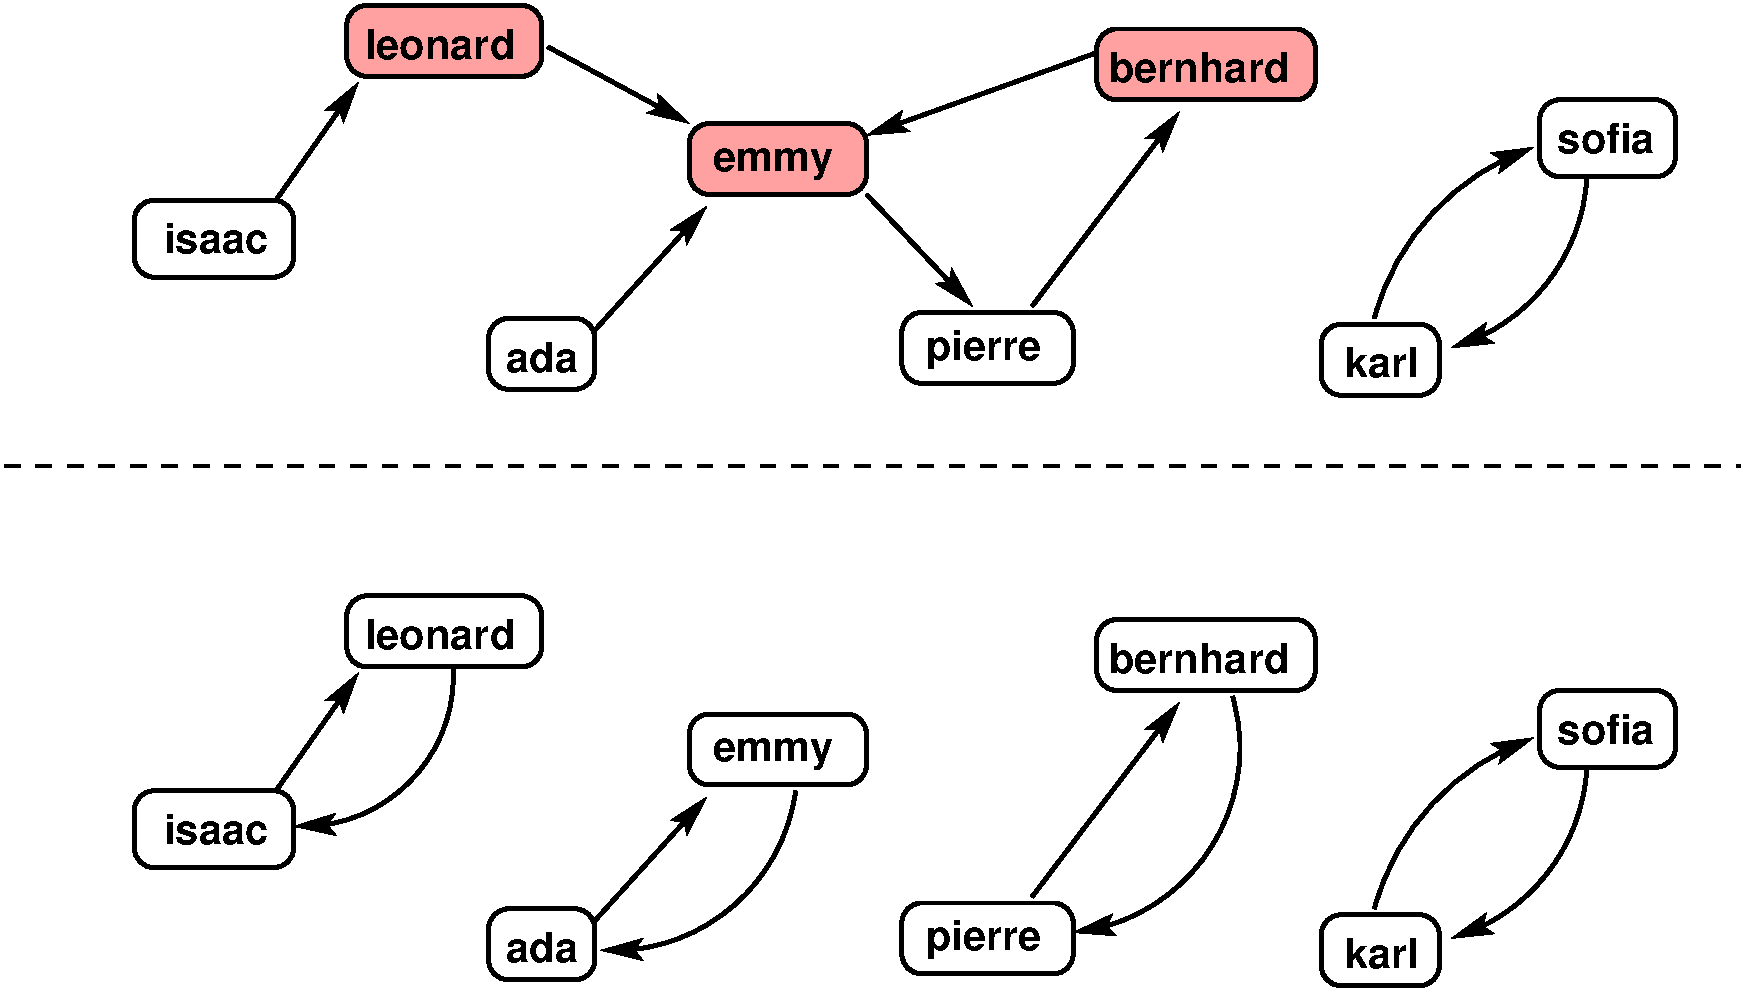
\includegraphics[width=0.5\textwidth]{polygonfig.pdf}
\end{center}

Pierwszy przykład jest zilustrowany na obrazku powyżej. Górna część pokazuje początkową sytuację miłosną,
gdzie strzałka z $s$ do $t$ oznacza, że $s$ początkowo kocha $t$, a różowym kolorem zaznaczone są
trzy postacie, które muszą zostać trafione strzałą amora w optymalnym (i unikatowym) rozwiązaniu.
Dolna część obrazka pokazuje sytuację po tych strzałach.

W drugim przykładzie (który spełnia ograniczenia trzeciego podzadania) jest kilka optymalnych rozwiązań.
Jednym z nich jest trafienie strzałą amora bohaterów \texttt{a}, \texttt{b} oraz \texttt{d} i spowodowanie, aby
zakochali się odpowiednio w \texttt{b}, \texttt{a} oraz \texttt{c}.

W trzecim przykładzie mamy miłosny trójkąt, dla którego niezależnie od tego, ile razy strzelimy strzałą Amora, zawsze ktoś zostanie samotny.
